\chapter{State of Art}
\label{chapter:SA}

This dissertation suggests the development of a conversational query builder that functions as a chat-based interface within the EHDEN project ecosystem. This interface aims to help researchers redefine their studies effectively. The conversational user assistant will return a query to help discover the best databases for a specific research. Studying state-of-the-art Information Retrieval systems to retrieve the most appropriate databases for a researcher's query is essential in this context. In addition, it is vital to explore Large Language Models, a recent advance of algorithms that are known for their language generation ability, and the actual state of conversational user assistants or chatbots. In the end, research about interactive query builder. And so these topics will be discussed below.


\section{Information Retrieval}

In computing and information science, {\ir} involves retrieving information from collections of unstructured data, such as documents. According to \citet{p_m_efficient_2021}, an {\ir} system requires input user queries and uses them to retrieve information from its collections, aligning with the users' needs. This process efficiently filters and narrows down the vast amount of available unstructured data, thereby preventing users from being overwhelmed by the sheer volume of data and aiding them in quickly accessing relevant and specific content.

In conformity with \citet{hambarde_information_2023}, conventional text retrieval systems were predominant in the initial stages of the {\ir} field. These systems mainly depended on matching terms between queries and documents. Nevertheless, these systems based on terms have limitations, including issues like polysemy, synonymy, and linguistic gaps, which may restrict their effectiveness.

With the advancement of technology, deep learning techniques emerged, improving conventional text retrieval systems and overcoming the constraints associated with term-based retrieval methods. For this reason, the performance of these systems increased significantly, resulting in a more accurate and streamlined retrieval of information for end-users \cite{hambarde_information_2023}.

In turn, deep learning methods have evolved. Neural Network Architectures, transfer learning, and pre-training techniques emerged. These approaches have advanced the representation of textual data and bolstered the {\ir} system's comprehension of natural language queries.

More recently, Transformer architectures with attention mechanisms have been implemented in {\ir} systems to enable more effective handling of complex queries and documents. Moreover, incorporating pre-trained (masked) language models like {\bert} \cite{devlin_bert_2018} and {\gpt}-2 has proven to enhance the performance of {\ir} systems, offering an advanced understanding and processing of context, capturing the relationships and nuances within the natural language query and the documents.

This field has many applications in the real world, such as search engines like Google, digital libraries, and e-commerce platforms. In compliance with \citet{p_m_efficient_2021}, {\ir} generally functions across three main scales: searching the web, retrieving personal information, and conducting searches for enterprises, institutions, and domain-specific contexts.

This section explores the {\ir} field, more specifically, traditional methods, neural {\ir} systems and how {\ir} can be joined with natural laguage.


\subsection{Traditional Methods}

Some successful classical methods are {\tfidf} and {\bm}, briefly explained next.

\subsubsection{TF-IDF}

To better understand the {\tfidf} method, first, it is necessary to understand the concepts of {\tf} and {\idf}. \citet{manning_introduction_2009} explained these concepts in their work. It is reasonable to assume that a document containing a query term more frequently is more relevant to that query. Therefore, it should be assigned a higher relevance and/or score. So, {\tf} is the number of term occurrences in a document. However, to evaluate the relevancy of a query, each term is regarded with equal importance, and this is the problem with the raw method explained above. \citet{manning_introduction_2009} clarified this with the following example: the automotive industry is expected to include the term "auto" in nearly every document. The  {\idf} calculates the rarity of a term across a set of documents. This measure is calculated as the logarithm of the inverse fraction of documents containing the term. The goal is to help prioritize some terms that are sporadic and possibly more informative.

The traditional {\ir} method, {\tfidf}, combines {\tf} and {\idf} definitions, as the name suggests, and then produces a weight for each term in each document, as \citet{manning_introduction_2009} and \cite{lan_research_2022} mention. Equation \ref{eqn:tfidf} shows that the weight is calculated as the product of {\tf} and {\idf} values, highlighting terms that are both important within a specific document and relatively uncommon in the document collection.

\begin{equation}
\textup{tf-idf}_{t,d} = \textup{tf}_{t,d} \times \textup{idf}_{t}.
\label{eqn:tfidf}
\end{equation}

\citet{manning_introduction_2009} noted the {\tfidf} weight assigned to a term in a document is highest when the term frequently appears in a few documents, providing discriminating solid power. The weight is lower when the term occurs less frequently in a document or is widespread across many documents, indicating a less pronounced relevance signal. The weight is at its lowest when the term is present in nearly all documents. However, {\tfidf} does not consider the semantic information of words, which limits its ability to accurately reflect the similarity between texts \cite{lan_research_2022}. To address this limitation, researchers have proposed hybrid methods that combine {\tfidf} with semantic understanding to calculate text similarity.

In summary, this {\ir} method evaluates the importance of a term within a document relative to its occurrence across a collection of documents.


\subsubsection{BM25}

{\bm}, the short form for Best Matching 25, is a ranking algorithm for {\ir} systems, especially in the context of search engines. \citet{hambarde_information_2023} noted that {\bm} and other initial retrievers are employed for their effectiveness in recalling pertinent documents from an extensive pool.

The core components of {\bm} include {\tf}, {\idf}, {\dl}, and tuning parameters. Recapping from the {\tfidf} section, {\tf} is the number of occurrences that a specific term is in a document, and {\idf} is a measure that indicates the importance of a term in the whole document. Equation \ref{eqn:bm25} gives the formula to calculate the {\bm} score.

\begin{equation}
score(D,Q) = \sum_{i}^{n} IDF(q_{i}) \ast \frac{f(q_{i},D) \ast (k1 + 1)}{f(q_{i},D) + k1 \ast (1 - b + b \ast \frac{fieldLen}{avgFieldLen})}.
\label{eqn:bm25}
\end{equation}

As \citet{phd_understanding_2023} explained, the {\bm} equation is composed of the ith query term (q) and the respective {\idf} and {\tf} values. Also, include a division between the {\dl}, represented in the formula as fieldLen, and the average document length, avgFieldLen. This ratio evaluates how much the length of the document field deviates from the average length. So, the \citet{noauthor_practical_2018} explained intuitively: a document tends to receive a lower score when it contains more terms, especially those that do not match the query. The value b is a fine-tuning parameter, and it is responsible for length normalization. When b is larger, the ratio has a more significant effect on the overall score. Finally, the k1 value means term frequency saturation. It is a fine-tuning parameter that prevents the term frequency component of BM25 from having an unlimited impact on the document score.

This algorithm is simple and effective in {\ir} tasks, mainly search tasks. Also, it can handle large collections. For these reasons, it is widely used and called a classic. However, {\bm} can not perform a semantic analysis of the query and the documents, so getting the context and, in turn, getting better results is challenging. 

% Another limitation is the ignorance of other crucial factors to get a better search beyond the factors relative to the {\tf} and {\dl}.


%% ponte de tradicionais para os mais recentes
While traditional information retrieval methods like {\tfidf} and {\bm} have been effective in matching queries to documents based on keyword frequencies and document lengths, the evolution of {\ai}, data complexity and user needs has led to the development of neural {\ir} systems.



\subsection{Neural Information Retrieval Systems}

Neural {\ir} systems represent a significant advancement in the field of {\ir}. Conforming to \citet{mitra_introduction_nodate}, these systems utilize neural network models and deep learning techniques to understand and interpret the semantic content of queries and documents, offering a more nuanced approach. Neural {\ir} systems can be broadly categorized into two types: Representation-based and Interaction-based models.

Conforming to \citet{chen_integrating_2023}, the representation-based model focuses on creating representations of both queries and documents. They employ techniques to convert text into high-dimensional vector spaces. In these spaces, semantically similar terms and phrases are represented by vectors that are close to each other, capturing the underlying meaning and relationships of words beyond their surface-level appearances. This approach utilizes architectures like {\rnn} and allows the system to understand the content of documents and queries on a deeper level. 

The interaction-based model examines how words in a query relate to words in a document, capturing complex patterns and dependencies between them \cite{chen_integrating_2023}. They often use attention mechanisms, as seen in Transformer-based models like {\bert}, to dynamically weigh the importance of different parts of the text based on their relevance to the query.

However, only the interaction-based model will be explored.

There are some approaches to adopting an interaction-based model. One of them is the Retrieval and Ranker. According to \citet{hambarde_information_2023}, this method can be separated into two stages, as the name suggests: Retrieval and Ranker. The following figure, adapted from \citet{hambarde_information_2023}, shows us an overview of interaction-based {\ir} systems, highlighting the two main stages.

\begin{figure}[ht]
    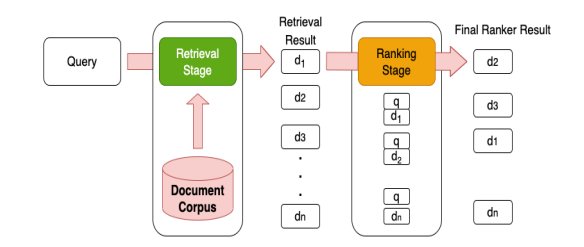
\includegraphics[width=14cm]{figs/chapter2/IR_system.png}
    \centering
    \caption{Overview of an interaction-based Information Retrieval model: Retrieval and Ranker.}
    \label{fig_ir_system}
\end{figure}

After analyzing the query, the retrieval stage will select an initial set of documents that are potentially pertinent to the query, as shown in figure \ref{fig_ir_system}. Subsequently, the relevance of these documents undergoes reassessment through the similarity scores. 

This is followed by the ranking stage, in which the primary objective is to adjust the order of the initially retrieved documents based on their relevance scores using a neural reranking, like {\bert} \cite{chen_integrating_2023}. This phase prioritizes the enhancement of result effectiveness rather than efficiency. In the end, it returns a rank of documents as close as possible to the user's query criteria. 


\subsection{Question Answering}

{\nlp} is the basis for building a {\qa} system, so it is important to give an overview of this technique. It is a field of {\ai} whose primary goal is to understand, interpret, and generate human language. The {\nlp} can be divided into two major components: {\nlu} and {\nlg}, according to \citet{ayanouz_smart_2020}

The \textbf{ {\nlu} } component is focused on enabling machines to understand and interpret human language in a meaningful way. {\nlu} involves processing and analyzing natural language data to comprehend its meaning, context, sentiment, and intent. 

In agreement with \citet{ngai_intelligent_2021}, the user queries can be processed by semantic analysis, pragmatic analysis, and syntactic analysis. \citet{ayanouz_smart_2020} explained these steps and added two more necessary steps to make it easier to understand: a lexical analysis and discourse integration.

\begin{itemize}
    \item \textbf{Lexical Analysis}: This step involves analyzing and identifying the structure of words. It breaks down the text into chapters, sentences, phrases, and words. \citet{chizhik_challenges_2020} defined lexical analysis as the pre-processing of the text following the steps: tokenization, removal of special characters, links, and punctuation, and removal of stop-words.

    \item \textbf{Syntactic Analysis}: The syntactic analyzer parses the grammar and arrangement of words, making the relationships between different words more explicit. Essentially, it rejects sentences with incorrect structures. This analysis can be seen as the process of normalizing tokens.

    \item \textbf{Semantic Analysis}: This step ensures the text is meaningful and interprets its correct meaning by mapping syntactic constructions. It ensures that only semantically valid content is retained. The recognition of entities is part of this analysis.

    \item \textbf{Pragmatic Analysis and Discourse Integration}: This step analyzes the overall context to derive the conclusive interpretation of the actual message in the text. It considers factors like the true meaning of a phrase or sentence based on the broader context.
\end{itemize}

The other component is \textbf{{\nlg}}. Language generation is responsible for crafting coherent and linguistically accurate responses. Simply put, it grapples with the challenge of navigating the intricacies of natural human language \cite{ngai_intelligent_2021}. 

Backtracking, {\qa} is a subfield of {\ir} and {\nlp}. According to \citet{zhong_building_2020}, {\qa} focuses on providing a single and specific answer to a question posed in natural language. Unlike {\ir}, which aims to return a broad range of relevant information or documents in response to a query, {\qa} seeks to pinpoint and provide one precise answer.

The traditional approach to question analysis and answering often involves mapping questions into predefined templates, such as "What-type" and "How-type". While widely utilized by existing online question-answering search engines, this template-based approach faces limitations in handling multiple questions \cite{zhong_building_2020}. 

So, with the advancement of technology, another approach emerged: deep learning-based question-answering. In contrast with the traditional approach, this approach employs deep learning techniques, like {\rnn}, to offer automatic representation and analysis of questions. These neural models, trained through end-to-end approaches, excel in extracting and understanding complex characteristics in textual documents.

Recently, deep learning approaches with attention mechanisms and transfer learning have enhanced the flexibility of representation in text classification and named entity recognition. \citet{zhong_building_2020} highlights {\bert} that has emerged as a powerful model, utilizing contextualized representations for transfer learning. {\bert}-based models showcase performance in question-answering tasks, even in domains like medicine.



\section{Large Language Models}
\label{llm}

It is crucial to trace briefly the development history to understand the concept of {\llm}. \citet{liu_prompting_nodate} explained this simply and intuitively.

Before {\llm}, there were only simple {\lm}, a subfield of {\nlp} and {\ai}, that have been called foundation models. A {\lm} is a statistical model used to predict the next word in a sequence of words. It calculates the probability of a given word occurring in a sequence, helping to determine which words are likely to appear next in a given context \cite{chang_language_2023}.

Most of these predictive models were based on probabilities and Markov assumptions, also known as {\slm}. This was heavily dependent on feature engineering. Afterward, as deep learning gained prominence, an architecture designed to learn data features automatically; in other words, neural networks for {\nlp} emerged to enhance {\lm}’s capabilities. Integrating feature learning and model training, {\nlm} established a comprehensive neural network framework applicable to diverse {\nlp} tasks \cite{liu_prompting_nodate}.

Most recently, the launch of the Transformer Block Architecture by \citet{vaswani_attention_2023} revolutionized this field. These deep-learning architectures led to the development of pre-trained models not explicitly designed for a particular task, including {\bert} and {\gpt}, collectively known as {\plm}. {\plm} have shown significant performance enhancements across various {\nlp} tasks.

Following this, the researchers have involved the scale of model parameters, and the paradigm of “Pre-train, Prompt, Predict" like \citet{liu_prompting_nodate} call, gained widespread acceptance. So, in terms of interaction with {\lm}, the prompts became crucial. Researchers name these {\plm} with hundreds of billions of parameters as {\llm}. Prompts effectively allow {\llm} to deal with a large number of complex and diverse tasks without a lot of effort.

This section discusses mainly {\llm}, exploring briefly their architecture and comparison between foundation {\llm}. Finally, it addresses some of its limitations.


\subsection{Definition}

{\llm} is an advanced {\lm} and belongs to generative {\ai}. It is designed to comprehend and generate text that is coherent and contextually relevant, engaging in human language interactions. Essentially, these advanced {\ai} systems mimic human intelligence. These models have a notable ability in natural language tasks, such as text generation and translation, {\qa}, decision-making, summarization, and sentiment analysis.

These models can process and predict patterns with accuracy. \citet{hadi_LLM_2023} combine sophisticated {\slm} and deep learning techniques to train, analyze, and understand huge volumes of data, learning the patterns and relationships among the data. For this reason, according to \citet{naveed_comprehensive_2023}, when provided with task descriptions and examples through prompts, {\llm} can produce textual responses to task queries. 

\citet{liu_prompting_nodate} say that the release of ChatGPT 1 garnered significant social attention, and research into {\llm} triggered more interest. This has led to the development of noteworthy products like PaLM, {\gpt}-2, {\gpt}-3, and, most recently, {\gpt}-4, and LLaMA and LLaMa-2.

{\llm} are revolutionizing {\nlp} and {\ai} research.


\subsection{Architecture Overview}

This subsection discusses the architecture of a {\llm}, which is supported by the Transformer Block architecture. Also, explains the pre-training process of this advanced {\lm}.

\subsubsection{Transformer Architecture}

The development and advancement of {\llm} is thankful for the introduction of Transformers by \citet{vaswani_attention_2023} in 2017. Most {\llm} are built on the Transformer model, which is based on a multihead self-attention mechanism and feedforward layers. This new technology enables parallelization and efficient handling of long-range dependencies, according to \citet{hadi_LLM_2023}, and led to the development of models that have achieved enormous results, such as {\gpt} by OpenAI and {\bert} by Google. The architecture of this revolutionized model is shown in figure \ref{fig_trans_arch}.

The innovation of this model is due to the multihead self-attention mechanism, one of the key components \cite{vaswani_attention_2023} \cite{hadi_LLM_2023}. It allows the model to weigh the importance of different words in a sequence when processing each word. This mechanism enables the model to focus on relevant information, capturing dependencies regardless of word order. 

However, the key advantage of this multihead self-attention mechanism is its highly parallelization \cite{vaswani_attention_2023}. This characteristic enables the Transformer model to be easily distributed and trained on a large scale using GPUs. The ability to parallelize computations means that Transformers can handle larger datasets and more complex tasks, unlike previous architectures like {\rnn}, where sequential processing of data was required.

Since the model doesn't have recurrence and convolution to understand the order of the input sequence, another component, Position Encoding, provides some information about the position of the tokens in the sequence. This is crucial for capturing sequential information in the data. 

\begin{figure}[ht]
    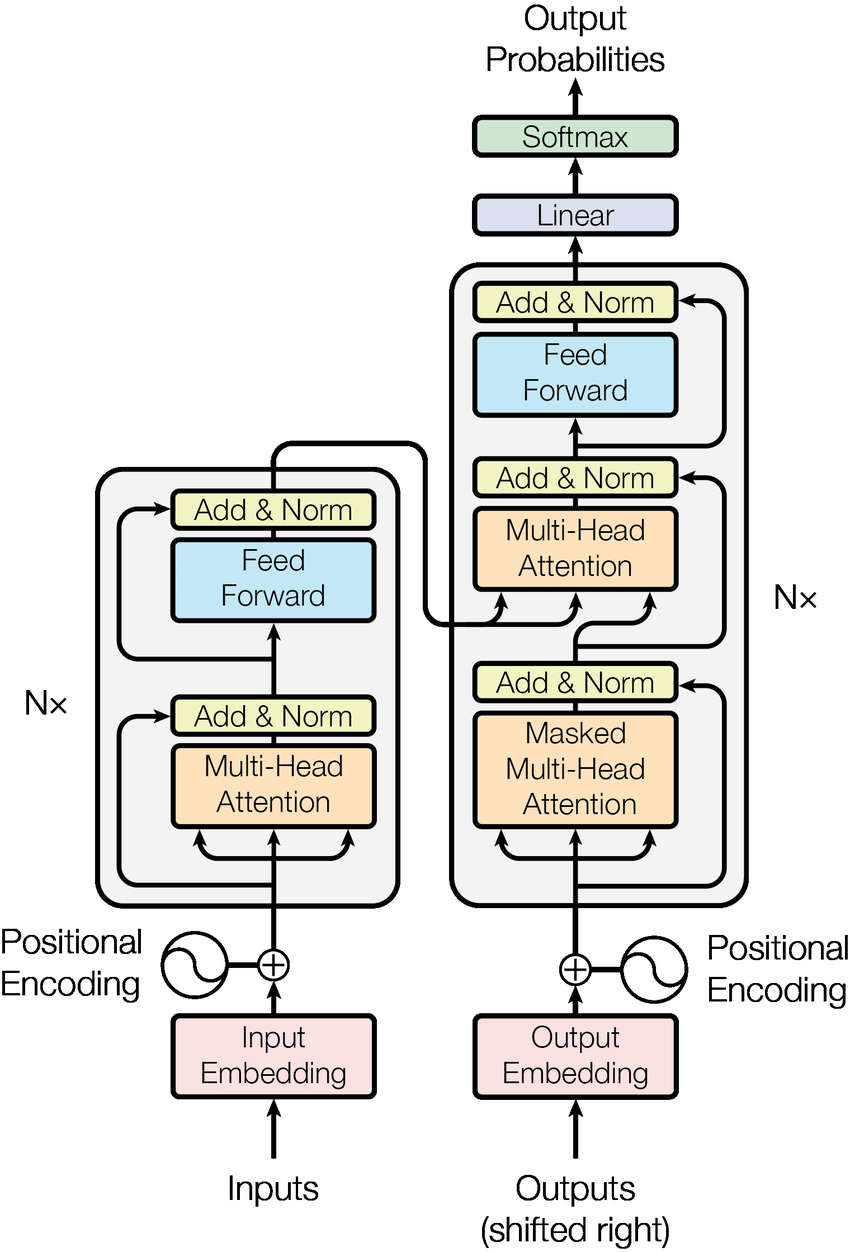
\includegraphics[width=8cm]{figs/chapter2/transformer.png}
    \centering
    \caption{The Transformer Block Architecture, from \citet{vaswani_attention_2023}.}
    \label{fig_trans_arch}
\end{figure}


\subsubsection{Pre-training Process}

Learning the patterns and relationships among the data starts with the pre-training process. In compliance with \citet{min_recent_pretrained}, first, the {\llm} needs to access a vast volume of textual data from multiple sources. The goal of this phase is to predict the succeeding word in a sentence based on the context given by the previous words through unsupervised learning. 

According to \citet{hadi_LLM_2023}, preparing and preprocessing the data before the training stage is necessary to achieve this. First, demand quality filtering from the training corpus. It is vital to remove unwanted, repetitive, duplicated, superfluous, and potentially harmful content from the massive text data. Next, it is necessary to pay attention to privacy. The data could have sensitive or personal information, so it is vital to address privacy concerns by removing this information from the pre-training corpus.

An important step, the tokenization, follows this \cite{hadi_LLM_2023}. This step aims to divide the unprocessed text into sequences of individual tokens, which are subsequently input into {\llm}. Moreover, it is vital in mitigating the computational load and enhancing efficiency during the pre-training phase. Figure \ref{fig_tokenization} visually presents the tokenization process \cite{noauthor_openai_nodate} carried out and explained by OpenAI.

\begin{figure}[ht]
    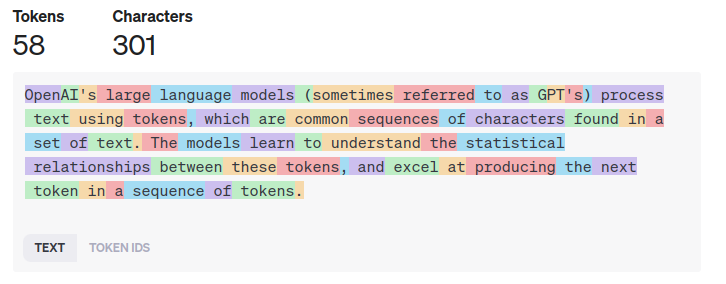
\includegraphics[width=14cm]{figs/chapter2/tokenization.png}
    \centering
    \caption{Tokenization process visually explained by OpenAI \cite{noauthor_openai_nodate}.}
    \label{fig_tokenization}
\end{figure}

After the pre-training process, the {\llm} goes through an optimization phase.


\subsection{Optimization Techniques}

There are some techniques to optimize the tasks and the accuracy of the {\llm}. Two of these techniques, Fine-tuning and Prompt Engineering, are explained next.


\subsubsection{Fine-tuning}

During pre-training, models are generally trained with the objective of next token prediction, learning the nuances of language structure and semantics. According to \citet{kamnis_generative_2023} and \citet{hadi_LLM_2023}, the fine-tuning phase involves adapting a pre-trained model to specific tasks and aligning it with human preferences, improving the performance on particular domains.

In this stage, the model is presented with labeled data to produce more contextually accurate responses for the specific task. Fine-tuning enables the {\llm} to specialize in diverse applications, ranging from language translation and question-answering to text generation. 

Some approaches could be applied to fine-tune the model. \citet{naveed_comprehensive_2023} distinguishes some of them, such as Parameter-Efficient Tuning. As {\llm} typically requires a lot of computational resources, like memory and computing, the Parameter-Efficient Tuning approach is helpful because it allows the model to train by updating fewer parameters, adding new ones, or selecting existing ones. Inside this approach, there are also some different methods. The commonly used indicated by \citet{naveed_comprehensive_2023} are Prompt Tuning, Prefix Tuning, and Adapter Tuning.

The Prompt Tuning method integrates trainable tokens, named soft prompts, to the beginning or within the input of a {\llm}, and only these tokens are adjusted during training to adapt the model for a specific task. This method keeps the rest of the model unchanged, ensuring the core knowledge and capabilities of the model are preserved while it learns to handle new types of requests or information.

In Prefix Tuning, a sequence of trainable tokens is introduced to transformer layers, with only the prefix parameters undergoing fine-tuning, while the remaining model parameters remain unchanged. These added prefixes function as virtual tokens, allowing input sequence tokens to attend to them during processing.

Meanwhile, in Adapter Tuning, small modules called adapters are added inside each layer of the Transformer. These adapters can be trained to adapt the model for specific tasks. The fine-tuning process works by slightly altering the model's internal features, allowing it to learn task-specific patterns without changing the entire model. LoRA (Low-Rank Adaptation) is one technique that implements Adapter Tuning, introduced by \citet{hu_lora_2021}. Instead of adding new layers like traditional adapters, LoRA learns low-rank matrices that are used to update the weights of the existing layers, maintaining the original weights of the model. This approach allows for efficient fine-tuning of the model on specific tasks while maintaining the model's original performance and avoiding significant increases in computational costs.


\subsubsection{Prompt Engineering}

With the emergence of {\llm}, other research fields were born. Prompt Engineering is one of these cases and has been widely applied. In compliance with \citet{mesko_prompt_2023} and \citet{ma_beyond_2023}, this emerging field involves designing, refining, and implementing prompts or instructions to direct the generated output of {\llm}, aiding in diverse tasks. {\llm} can follow specific directions provided by users in natural language after being tuned with instructions.

There are some techniques of prompt engineering, such as Chain of Thought (CoT) and Reason-Action (ReAct). 

CoT is a popular problem-solving approach for prompt engineering that aims to break complex tasks into multiple and simpler subtasks and solve them. So, \citet{wei_chain--thought_2023} explained that this method involves explicitly modeling the reasoning processes that lead to a final answer, rather than directly generating an answer. This explanation of reasoning often leads to more accurate results. Figure \ref{fig_cot} explains the effect of this technique.

ReAct is a prompt technique introduced by \citet{yao_react_2023}. The idea behind this is to simultaneously include both reasoning and action within a single prompt. To solve a complex task, ReAct consists of three tasks for every subtask: 1) \textbf{Reason} involves analyzing the current situation and determining the necessary steps; then, 2) \textbf{Action} entails executing a task based on the reasoning. 3) \textbf{Observation} then refers to examining the outcomes following the action.


\begin{figure}[ht]
    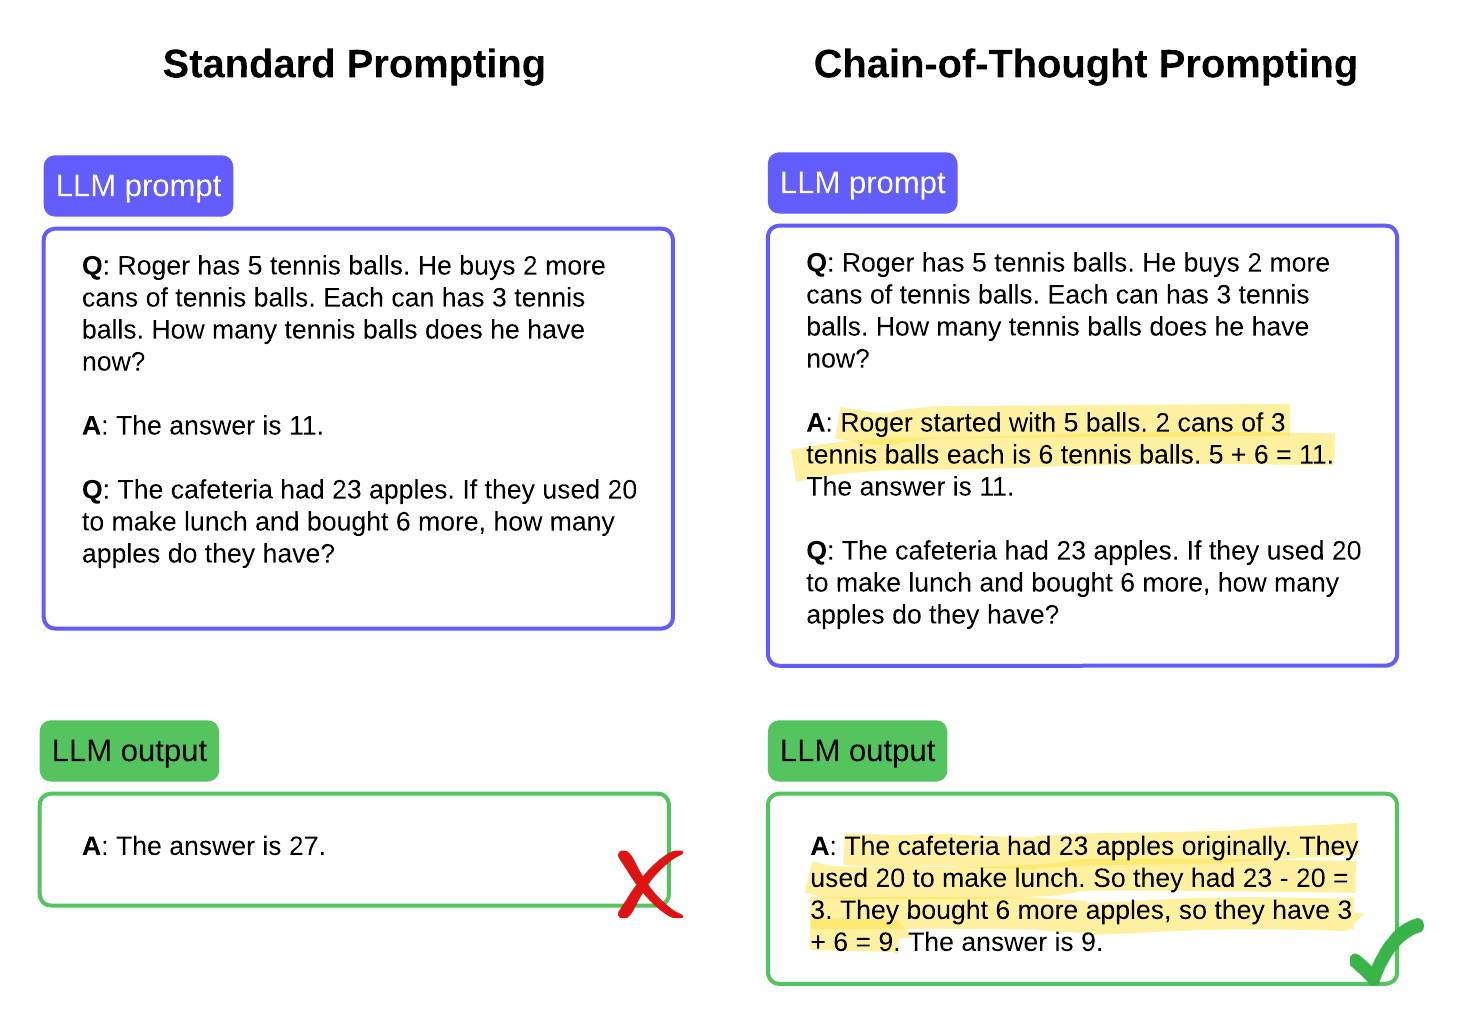
\includegraphics[width=14cm]{figs/chapter2/CoT.png}
    \centering
    \caption{Example of Chain-of-thought prompting. The reasoning processes are highlighted in yellow. Adapted from \citet{wei_chain--thought_2023}.}
    \label{fig_cot}
\end{figure}


\citet{mesko_prompt_2023} raise a series of recommendations for more effective {\llm} prompts: it must be as precise as possible; providing the setting and the context of the question is essential; describe the goal of the prompt first; give a role to the {\llm} to get more context (for example, "You are a math teacher and explain the natural numbers"); continuous {\llm} prompt refinement; prefer open questions over close-questions. Regularly testing prompts in real-world situations is crucial, as their effectiveness is most accurately assessed through practical application.



\subsection{Comparison between foundation Large Language Models}

The best way to compare {\llm} is to evaluate the model's performance. \citet{hadi_LLM_2023} identified five factors to make this comparison: the size of the training corpus, the quality of the training corpus, the number of parameters, the complexity of the model, and some test tasks.

The primary foundation models of {\llm} are {\gpt}-4 by OpenAI, LLaMA 2 by Meta, PaLM 2 by Google, and Falcon by Technology Innovation Institute (TII). These {\llm} are provided by big companies and have outstanding progress in the evolution of this area. These models gave rise to many others.

LLama 2 is an open source {\llm} by Meta (\citet{touvron_llama_2023}). LLaMa 2 was trained on 40\% more data than LLaMa 1, the model from which it came, and has double the context length. So, the model size of LLaMa 2 is 7 billion, 13 billion, or 70 billion parameters. With 4096 context length and trained on 2 trillion pretraining tokens, this {\llm} is commonly fine-tuned for chat use cases. Many other models, like Alpaca, Vicuna, and Llama-2-chat, came from LLaMa and deserve further analysis. It is accessible for both research and commercial purposes

The recent {\gpt} model from OpenAI, {\gpt}-4, is a closed source {\llm} (\citet{openai_gpt-4_2023}). Trained on a meticulously curated dataset from various textual sources, including books, articles, and websites, {\gpt}-4 exhibits remarkable performance with text and image inputs. It is the {\llm} behind ChatGPT. It has 32 000 context length. OpenAI has chosen to provide limited technical details about the training methodology used for this advanced model, including specific information on parameter counts.

The Google generative chatbot, Bard, uses as {\llm} the PaLM 2 model developed by Google (\citet{anil_palm_2023}). It emerged from PaLM with 540 billion parameters. PaLM 2 is a closed source {\llm}, and, following the OpenAI approach, has opted to disclose limited technical specifics, including the number of parameters. 

The Falcon {\llm} is an open-source model with impressive performance and scalability (\citet{almazrouei_falcon_2023}). There are three variations of the model size: 7 billion, 40 billion, and the most recent, 180 billion of parameters. This Falcon 180B is equipped with an impressive 180 billion parameters and trained on 3.5 trillion tokens. It is accessible for both research and commercial purposes.

The table \ref{table:comparison} summarizes the important aspects of comparison between this foundation {\llm}.

\begin{table}[ht]
    \scalebox{0.8}{
        \begin{tabular}{|c|c|c|c|c|c|c|}
        \hline
        \textbf{Model} & \textbf{Provider} & \textbf{\begin{tabular}[c]{@{}c@{}}Model size\\ (Parameters)\end{tabular}} & \textbf{Context Length} & \textbf{Tokens} & \textbf{Fine-tuneability} & \textbf{Open-source} \\ \hline
        GPT-4          & OpenAI            & -                                                                          & -                       & -               & No                        & No                   \\ \hline
        LLaMa 2        & Meta              & 7B, 13B, 70B                                                               & 4096                    & 2T              & Yes                       & Yes                  \\ \hline
        PaLM 2         & Google            & -                                                                          & -                       & -               & No                        & No                   \\ \hline
        Falcon         & TII               & 7B, 40B, 180B                                                              & 2048                    & 3.5T            & Yes                       & Yes                  \\ \hline
        \end{tabular}
    }
    \caption{Comparison of foundation Large Language Models.}
    \label{table:comparison}
\end{table}



\subsection{Limitations}

It is safe to say that {\llm} are significantly impacting the world. According to \citet{liu_prompting_nodate}, this is justified by their abilities, mainly in-context learning, reasoning for complex content, instruction following, and creative capacity.

However, {\llm} has some limitations. \citet{hadi_LLM_2023} address some of them, and the most important ones are biased responses, hallucination, explainability, and cyber-attacks. 

We already know that {\llm} are pre-trained with extensive training data. But suppose that data contains some biased information related to factors such as gender, socioeconomic status, and/or race. In that case, this may result in analyses and recommendations that are discriminatory or inaccurate across diverse domains. The problem of bias applies not only to training data but also to user interaction bias, algorithmic bias, and contextual bias. The user interaction bias means that, as user prompts shape responses, and if users consistently ask biased or prejudiced questions, the model may acquire and reinforce these biases in its replies.

A severe limitation that is an active area of research is hallucination. \citet{church_emerging_2023} characterized {\llm} hallucinations as when the model attempts to fill gaps in knowledge or context, relying on learned patterns during training. Such occurrences can result in inaccurate or misleading responses, detrimental to the user and the model's reliability.

The way the {\llm} makes decisions is unknown. Comprehending the decision-making process of a complex model with billions of parameters, like {\llm}, is challenging. So, the explainability of these models is a big limitation \cite{hadi_LLM_2023}. Sometimes, it is necessary to decipher the factors that influenced an {\llm}'s decision and this limitation poses difficulties in offering a clear and concise explanation. In vital sectors like healthcare, where decisions carry substantial consequences, ensuring transparency and the capability to elucidate the model's predictions is essential.

Another limitation is the cyber-attacks. A {\llm} can suffer some prompt injections from a malicious user to extract sensitive information from the model, according to \citet{kshetri_cybercrime_2023}. This is called the Jail Break attack \cite{hadi_LLM_2023}. Another attack is Data Poisoning Attacks, which consist of data poisoning strategies to manipulate the model's output.

Furthermore, \citet{liu_prompting_nodate} highlighted another limitation: the temporal lag of the training corpus. {\llm} cannot retrieve information in real time, and the answer generated may not be the most current.

It is important to be aware of these limitations.


\section{Conversational User Assistants}

Conversational User Assistants, also known as chatbots, chatterbots, or virtual assistants, have become a vital aspect of the digital landscape. These tools are generally dialogue systems that understand, interpret, and generate human language, enabling them to communicate with users to dissolve their questions.

Chatbots are increasingly being used in various contexts due to their many benefits. These aspects that make companies bet on the use of chatbots are the continuous availability to support and assist the customer, ensuring more consistent support; the cost-efficiency by reducing the human customer support; the time-saving both for the organization and for customers due to the immediate responses to the user queries; the ease and intuitiveness of this systems; and, improve service with every interaction \cite{misischia_chatbots_2022}. Because of this, the utility of the chatbots as tools is increasing as the technology advances. 

The rise of conversational user assistants is underpinned by a convergence of technologies, specifically by {\llm}.

This section provides a brief overview of chatbots, followed by an in-depth focus on Generative-Based Chatbots. It encompasses important concepts from their definition to some techniques employed in their development and optimization.


\subsection{Overview of Conversational User Assistants}

To provide a comprehensive understanding of conversational user assistants, it's crucial to first explore some of their characteristics, such as domains and method of response generation.

\citet{nuruzzaman_survey_2018} defined the differences between chatbots with opened or closed domains. In an open-domain environment, conversations can go in any direction without a predefined goal or intention. Conversely, in closed-domain environments, the conversation is centered on a particular topic. A closed-domain chatbot is designed with a clear objective.

It is important to differentiate chatbots in their way of giving or generating a response based on an input query. \citet{peng_survey_2019} distinguish three main types of chatbots based on their response generation: Rule-based, Retrieval-based and Generative-based chatbots.

A \textbf{rule-based chatbot} examines fundamental features of the user's input statement and generates a response based on a predefined set of manually crafted templates. This type is more applicable in a closed-domain conversation. ELIZA, introduced by \citet{weizenbaum_elizacomputer_1966}, was the first chatbot that applied this primitive technique.

A \textbf{retrieval-based chatbot} picks a response from an extensive precompiled dataset. It selects the most promising reply from the top-k ranked candidates. Thus, they refrain from producing new text. It has limited flexibility regarding closed-domain and in terms of errors \cite{agarwal_review_2020}.

A \textbf{generative-based chatbot} generates a text sequence as a response rather than choosing it from a predefined set of candidates. These chatbots are very flexible and can handle open domains because they are implemented with deep learning techniques. The interactions will be more identical to those of humans, as it implements a self-learning method from a large quantity of interaction data \cite{peng_survey_2019} \cite{agarwal_review_2020}. However, this could be complex and costly to implement.

The only type that will be covered will be generative chatbots, due to their capabilities.


\subsection{Generative-Based Chatbot}

Generative-based conversational user assistants are chatbots that use generative models to generate natural language responses. These chatbots utilize sophisticated deep-learning techniques, such as {\llm}. {\llm}, as described in section \ref{llm}, has the ability to understand and generate human-like text in context. This advanced {\lm} has been widely used in the modern chatbots. ChatGPT is an example of this type of chatbot.

Although an {\llm} can generate text from a query, it is not prepared to be applied to a chatbot. There are some techniques for improving and optimizing the model to behave like a chatbot, such as {\rlhf}.

In addition, some techniques aim to combat some of the limitations of chatbots, such as hallucination, by increasing their knowledge, such as {\rag}.

The {\rlhf} and {\rag} are explained in more depth below.


%%%%%%%%%%%%%%%%%%%%%%%%%%%%%%%%%%%%%%%%% commented %%%%%%%%%%%%%%%%%%%%%%%%%%%%%%%%%%%%%%%%%
\iffalse       

There are some methods to improve the results of a {\llm} used on chatbot: fine-tuning the {\llm}, {\rag}, and Prompt Engineering.

\begin{table}[ht]
    \centering
    \begin{tabular}{|cc|cc|}
    \hline
    \multicolumn{2}{|c|}{\multirow{2}{*}{\textbf{}}}                                                                                 & \multicolumn{2}{c|}{\textbf{Model Adaptation Required}}                                                                   \\ \cline{3-4} 
    \multicolumn{2}{|c|}{}                                                                                                           & \multicolumn{1}{c|}{Low}                                                                             & High               \\ \hline
    \multicolumn{1}{|c|}{\multirow{2}{*}{\textbf{\begin{tabular}[c]{@{}c@{}}External \\ Knowledge \\ Required\end{tabular}}}} & Low  & \multicolumn{1}{c|}{Prompt Engineering}                                                              & Fine-tuning        \\ \cline{2-4} 
    \multicolumn{1}{|c|}{}                                                                                                    & High & \multicolumn{1}{c|}{\begin{tabular}[c]{@{}c@{}}Retrieval-Augmented \\ Generation (RAG)\end{tabular}} & All of the methods \\ \hline
    \end{tabular}
    \caption{Optimization methods of generative-based chatbots.}
    \label{table:optimization}
\end{table}

The table \ref{table:optimization} shows how these methods influence model adaptation and external knowledge. Mixing all methods requires a high model adaptation and external knowledge, but provides better results. 

\fi
%%%%%%%%%%%%%%%%%%%%%%%%%%%%%%%%%%%%%%%%% commented %%%%%%%%%%%%%%%%%%%%%%%%%%%%%%%%%%%%%%%%%


\subsubsection{Reinforcement Learning from Human Feedback (RLHF)}

In the context of {\ai}, according to \citet{li_human-centered_2019}, {\rlhf} is a popular approach in which an agent learns how to perform a task based on evaluative feedback provided by a human observer.

{\rlhf} in generative-based chatbots is a topic that has been explored in the field of conversational {\ai}. This technique is a transformative technique that combines reinforcement learning and supervised learning to refine {\llm} for chatbot applications. \citet{tran_enhancing_2023} stated that {\rlhf} aims to align chatbot responses to human preferences, improving chatbots' performance and making them more human-like.

The process encompasses several crucial stages, in conformity with \citet{axelsson_modeling_2022}. Initially, the {\llm} is pre-trained on a large dataset of text, which allows it to learn a wide range of language patterns and knowledge. After pre-training, the model undergoes a phase of supervised fine-tuning. In this phase, the {\llm} is trained on a dataset of conversational examples that are specifically curated to reflect the desired outputs for the chatbot. 

After that, humans provide feedback on the model's outputs. This feedback is crucial because it is used to build and train a reward model. The reward model learns to predict the quality of the model's responses based on the human-provided feedback \cite{axelsson_modeling_2022}.

The {\llm} is further fine-tuned using reinforcement learning, where it learns to generate responses that maximize the predicted reward, using the reward model created in the previous phase. This stage enables the model to optimize its responses through the reward model, which is based on human feedback.

The process often involves several iterations of feedback and fine-tuning to continually improve the chatbot's performance. This can resolve errors, improving the refining the conversational style.



\subsubsection{Retrieval-Augmented Generation (RAG)}
\label{rag_section}

{\rag} is a subfield of {\nlp} and {\ai}. This approach was introduced by \citet{lewis_retrieval-augmented_2020} in 2020 and combines retrieval-based and generative models to enhance content generation and information retrieval processes. For a clearer comprehension of this method, \citet{gao_retrieval-augmented_2023} made a survey into {\rag} systems and distinguish the parametric knowledge from non-parametric knowledge. 

Traditionally, {\llm} can adapt their knowledge and responses to a specific domain by fine-tuning models with parameters. This is \textbf{parametric knowledge} because the {\llm} knowledge is provided through the model's training data. However, entirely parameterized {\llm} have limitations, including data not currently updated and hallucinations. The \textbf{non-parametric knowledge}, provided by external information sources, emerged to solve these limitations. This non-parametric knowledge approach is known as {\rag}. 

So, according to \citet{lewis_retrieval-augmented_2020}, {\rag} involves retrieving pertinent information from external knowledge bases, giving more context to the {\llm}. This enables the {\llm} to access and utilize up-to-date and/or domain-specific information to enhance response accuracy and relevance. This process leads to reducing hallucinations.

The figure \ref{fig_rag} shows the workflow of a {\rag}. This model aims to retrieve relevant information from an extensive corpus of documents when answering questions, subsequently adding this information in the prompt as context to enhance the quality of predictions in compliance with \citet{lewis_retrieval-augmented_2020}.

%% FIXAR ESTA IMAGEM
% image reference: https://towardsdatascience.com/retrieval-augmented-generation-rag-from-theory-to-langchain-implementation-4e9bd5f6a4f2
\begin{figure}[ht]
    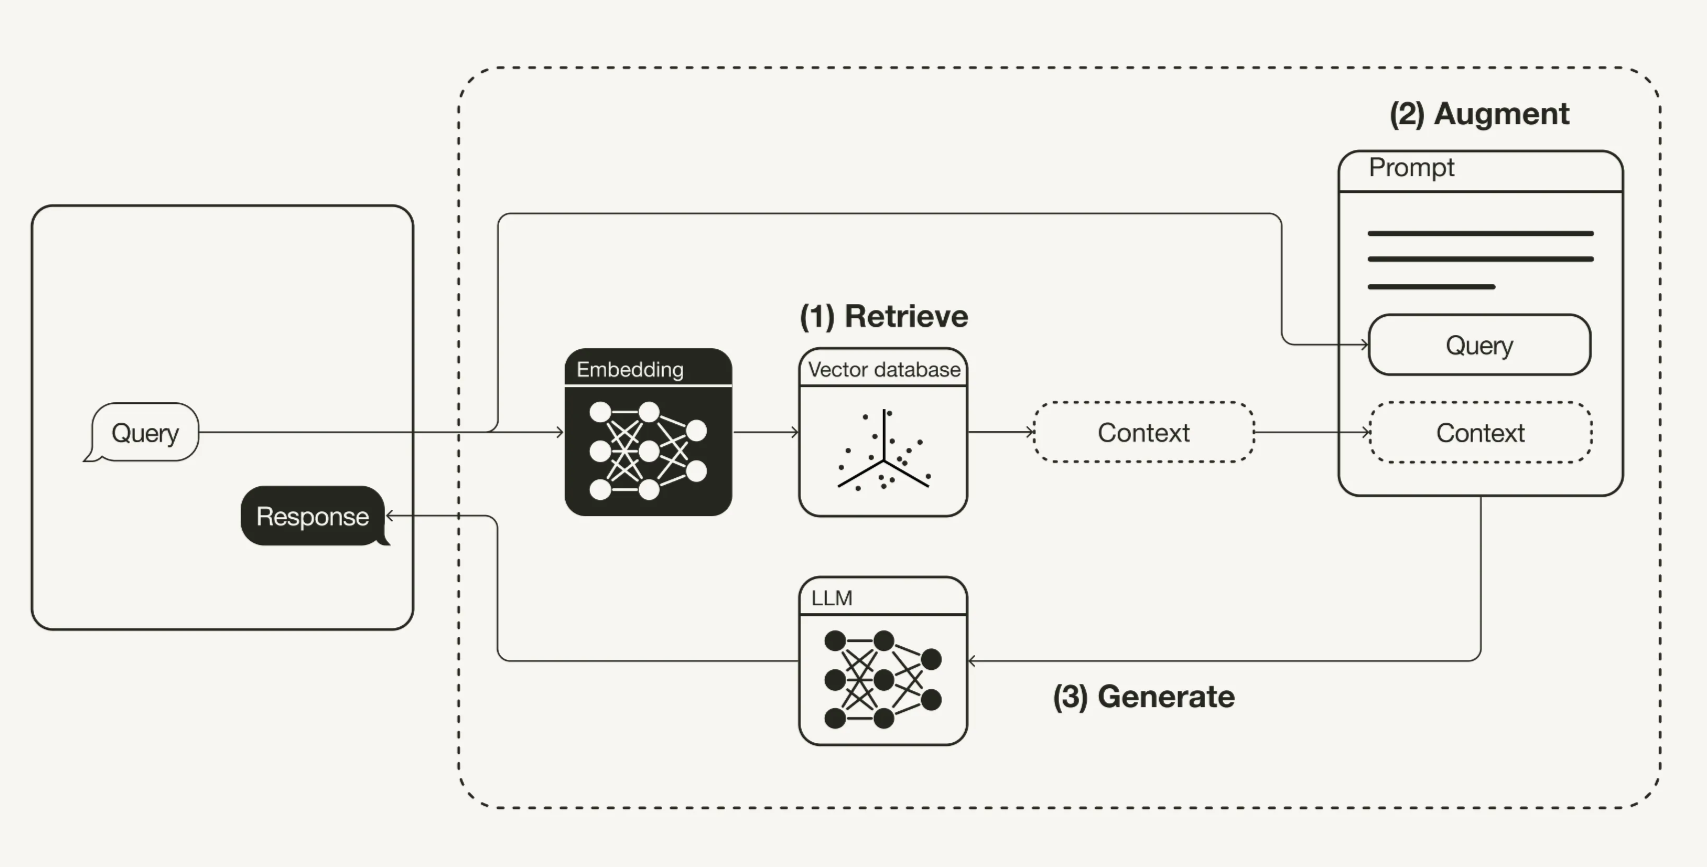
\includegraphics[width=14cm]{figs/chapter2/rag_workflow.png}
    \centering
    \caption{Retrieval-Augmented Generation Workflow.}
    \label{fig_rag}
\end{figure}


\citet{gao_retrieval-augmented_2023} explain simply the workflow. The first step is 1) Retrieve information from an external data source, such as a vector database, as in the example in figure \ref{fig_rag}. This step utilizes {\ir} models, such as {\bm}, to retrieve relevant information based on the query. The second step is 2) Augment, improving the {\llm} prompt with the context retrieved in the previous stage. The last step is 3) Generation. Using the prompt with context, the {\llm} generates a response to the query, based on the external information retrieved.

% escrever mais? vantagens,  RAG vs Fine-tuning, tipos de RAG


\section{Interactive Query Builder}

A query builder is a user interface tool for dynamically searching and filtering database objects, constructing a query according to user preferences, as the work of \citet{mussa_forestqb_2022} shows. This query could be in different formats, such as SQL and JSON. This tool lets users construct queries visually, eliminating manual research or coding. 

This section is particularly significant as there is limited documentation on conversational query builders. Therefore, it documents the general workings of query builders and delves into a detailed explanation of the functioning of the ATLAS cohort definition.

\subsection{General Query Builders}

% explicar como funcionam de forma geral

Users interact with the query builder through a user-friendly interface. Figure \ref{fig_query_builder} shows a query builder interface from jQuery QueryBuilder \cite{noauthor_jquery_nodate}.

\begin{figure}[ht]
    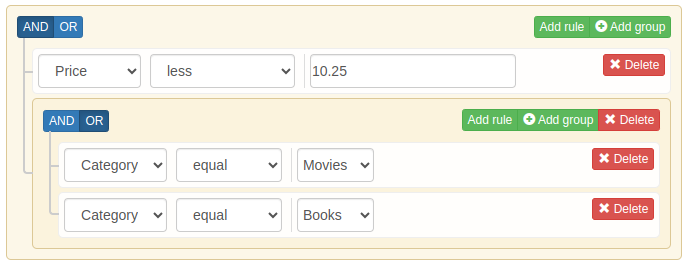
\includegraphics[width=14cm]{figs/chapter2/querybuilder.png}
    \centering
    \caption{Query builder from jQuery QueryBuilder \cite{noauthor_jquery_nodate}.}
    \label{fig_query_builder}
\end{figure}

Users can add rules and conditions/groups with some clicks. Each rule typically consists of a field, an operator, and a value. The conditions/groups could be an AND or an OR. Using figure \ref{fig_query_builder} as an example, there is a group with two elements joined with a condition AND: a rule and another group. This other group is composed of two rules joined with a condition OR.

As users build their queries, the query builder internally represents the conditions in a structured format, often a structured JSON of rules and groups, that reflects the logical structure of the query \cite{noauthor_jquery_nodate}.

In summary, a query builder simplifies creating complex queries by providing a visual and interactive interface, making it more accessible \cite{noauthor_introducing_2021}.

There are several advantages of its use \cite{noauthor_introducing_2021}: offers a user-friendly interface with menus, operators, and suggestions to facilitate the creation of accurate queries; users, often without direct permissions to modify the data source, can leverage the query builder to transform datasets without making changes to the underlying database; and, the generated queries are easily modifiable, allowing for flexibility in adjustments or repetitions.


\subsection{ATLAS}
\label{atlas}

% explicar como funciona o processo

ATLAS, an open-source and web-based software application, is freely accessible and was created by the {\ohdsi} community. It aids in helping researchers conduct scientific analyses on standardized observational data converted to the {\omop}.

Using healthcare claims data, researchers can define cohorts by categorizing groups of people according to their exposure to a medication or their diagnosis of a certain health condition. ATLAS offers the functionality to search medical concepts, enabling the identification of cases with particular conditions or drug exposures. Moreover, it allows for the examination of patient profiles within a given cohort, providing a way to visualize the healthcare records of specific subjects.

There are some different definitions of cohort, but, in the {\ohdsi} research, according to \citet{informatics_chapter_nodate}, a cohort is a query that defines a set of persons who meet certain inclusion criteria over a specified duration.

Cohorts serve as fundamental units for addressing research questions. A key characteristic of these cohorts is their independent definition. The distinct structure facilitates their reuse across different research contexts.


\subsubsection{Cohort definition}

There are two approaches to building a cohort: rule-based and probabilistic. The most popular one is the rule-based cohort definition, which uses explicit rules to describe when a patient is in the cohort.

In ATLAS, the process of defining a cohort is composed of 3 stages \cite{informatics_chapter_nodate}: Cohort Entry Events, Inclusion Criteria, and Cohort Exit.

The creation of a cohort starts with \textbf{Cohort Entry Events}, defining the initial event criteria. This involves the primary identification of the population of interest, which might include users of a certain drug, individuals with a specific diagnosis, or a combination of factors. 

The concept set needs to be specified in the Cohort Entry Events. It is a collection of standardized medical concepts used to define clinical elements like diseases, drugs, or procedures. For instance, if the study is about diabetes, the concept set will include various codes representing diabetes in different medical terminologies. These sets ensure that the cohort captures all relevant instances of the condition or exposure across different healthcare data sources.

Additional initial event criteria can also be added to refine the population further, such as the event occurring within a certain time frame.

After defining the initial event, the next step is to establish \textbf{Inclusion Criteria}. These criteria are based on a combination of domain-specific attributes to further refine and specify the cohort population, ensuring that it aligns closely with the research objectives. The inclusion criteria can be based on a range of factors such as age limits, the presence of certain symptoms, or a specified duration of medication use.

Finally, defining the \textbf{Cohort Exit} criteria is crucial for determining when individuals no longer belong to the cohort. This stage is important for studies where the duration of membership in the cohort is relevant to the research question.

In compliance with \citet{informatics_chapter_nodate}, a well-defined cohort specifies how a patient enters a cohort and how a patient exits a cohort.

After defining the cohort, it is possible to generate an SQL code with the query to get the list of individuals who meet the criteria. ATLAS also facilitates the reuse of cohort definitions across different studies by allowing users to export and import cohort definitions in JSON format. This enhances the efficiency and reproducibility of research within the OHDSI network.

A cohort definition can be seen as a query builder, a little different when compared to other general query builders.

% meter uma imagem da interface ?


\section{Summary}

To sum up, the proposed query builder is a generative-based chatbot with a closed domain. Closed-domain chatbots are specialized in specific areas, offering precise responses. Generative chatbots use advanced {\lm} to create dynamic responses closer to human interactions.

The utilization of {\llm} allows improvements in the {\nlg} capabilities of chatbots and guides conversations more effectively, especially in the task of defining cohorts in medical research. LLaMa-2 and Falcon appear to be good options to implement since they are open-source and have the possibility of fine-tuning the model. Fine-tune has the role of optimizing chatbot performance, alongside Prompt engineering and {\rag}. However, for this specific case, I don't think much external knowledge will be needed, so the use of fine-tuning should be enough.

In terms of {\ir}, in order to retrieve the most interesting databases according to the user's needs, the {\bm} technique proves to be a good balance between effectiveness and efficiency. {\bm} is a sophisticated yet relatively straightforward algorithm that improves upon the traditional {\tfidf} approach. Neural {\ir} systems, like Interaction-based models, show good results in the {\ir} tasks, but are complex and the neural networks require substantial computational power. It is a lot simpler to implement than the Neural {\ir} systems, as well as requires fewer computer resources. 

ATLAS by OHDSI provides a cohort definition, which is a query builder to define groups of people based on the research question using healthcare claims data. However, the interface revealed not very user-friendly and intuitive because it requires the user to have a good knowledge of its use and important concepts. Therefore, a chatbot that builds a cohort definition improves the user experience by making it more intuitive and autonomous.


%  meter mais referencias e citações